% \documentclass{book}

\documentclass[12pt]{article}
\usepackage[pdfborder={0 0 0.5 [3 2]}]{hyperref}%
\usepackage[left=1in,right=1in,top=1in,bottom=1in]{geometry}%
\usepackage[shortalphabetic]{amsrefs}%
\usepackage{amsmath}
\usepackage{enumerate}
\usepackage{enumitem}
\usepackage{amssymb}                
\usepackage{amsmath}                
\usepackage{amsfonts}
\usepackage{amsthm}
\usepackage{bbm}
\usepackage[table,xcdraw]{xcolor}
\usepackage{tikz}
\usepackage{float}
\usepackage{booktabs}
\usepackage{svg}
\usepackage{mathtools}
\usepackage{cool}
\usepackage{url}
\usepackage{graphicx,epsfig}
\usepackage{framed}
\usepackage{hyperref}  

\def\noi{\noindent}
\def\T{{\mathbb T}}
\def\R{{\mathbb R}}
\def\N{{\mathbb N}}
\def\C{{\mathbb C}}
\def\Z{{\mathbb Z}}
\def\P{{\mathbb P}}
\def\E{{\mathbb E}}
\def\Q{\mathbb{Q}}
\def\ind{{\mathbb I}}

\graphicspath{ {images/} }

\begin{document}

\title{}
\author{\vspace{-10ex} }

\begin{center}
{\LARGE APMA 1650 -- Homework 2}\\
\vspace{5mm}
{\large Due Thursday, July 7, 2016}\\
\vspace{5mm}
Homework is due during class or by 3:45 pm in the homework drop box in 182 George St.\\
Show all of your work used in deriving your solutions.
\end{center}

\begin{enumerate}

\item You have a bag containing $r$ red marbles and $g$ green marbles. (Both $r$ and $g$ are positive integers.) You draw marbles from the bag, but there is a twist! Each time you draw a marble from the bag, you replace it with along with another marble of the same color. (You never run out of marbles to add to the bag.)
\begin{enumerate}
\item What is the probability of getting a red marble on the first draw?\\

Since there are $r$ red marbles and $r + g$ total marbles, and there is equal probability of drawing any marble, the probability of a red marble on the first draw is $r / (r + g)$.

\item What is the probability of getting a red marble on the second draw? \\

You can do this with the law of total probability. Let $R_1$ and $G_1$ be the events that we draw red or green on the first draw, and $R_2$ and $G_2$ be the events that we draw red or green on the second draw. We are interested in $\P(R_2)$. Note that $\{R_1, G_1\}$ is a partition of the sample space, since our first draw must be either red or green. Using the law of total probability with this partition, and filling in the appropriate probabilties based on what happens to the bag after the first draw:
\begin{align*}
\P(R_2) &= \P(R_2|R_1)\P(R_1) + \P(R_2|G_1)\P(G_1) \\
&= \frac{r+1}{r+g+1}\frac{r}{r+g} + \frac{r}{r+g+1}\frac{g}{r+g}\\
&= \frac{(r+1)r + rg}{(r+g+1)(r+g)}\\
&= \frac{r(r+g+1)}{(r+g+1)(r+g)}\\
&= \frac{r}{r+g}
\end{align*}
which is the same probability as for the first draw! If you prefer, you can do this with a tree diagram, which gives the same result. 

\item Make a guess for the probability of getting a red marble on the $n$th draw.\\

If the first two draws have the same probability of getting a red marble, it stands to reason that \emph{every} draw will have the same probability of getting a red marble, so we will guess that the probability of a red marble on the $n$th draw is also $r / (r + g)$. This can be proven by induction.
\end{enumerate}

\item You have $m$ red marbles which you will put uniformly at random into $n$ boxes. What is the expected number of boxes which are empty after all $m$ marbles have been distributed. \\

Let $X$ be the number of empty boxes. Since there is no essential difference between the boxes (we can swap them around without affecting the expected value), since we are looking for an expected value, and since the expected value involves counting these boxes, we will use the method of indicator random variables together with linearity of expectation. Define the indicator random variables $X_i, i = 1, \dots, n$, where
\[
X_i = \begin{cases}
0 & \text{box $i$ is empty}\\
1 & \text{box $i$ is not empty}
\end{cases}
\]
Then since $X$ counts the number of empty boxes, $X = X_1 + \cdots + X_n$. By linearity of expectation:
\[
\E(X) = \E(X_1 + \cdots + X_n) = \E(X_1) + \cdots + \E(X_n)
\]
Now we look at one of the terms in the sum on the right. Let's evaluate $\E(X_i)$ for some box $i$. By the definition of the expected value of a discrete random variable,
\begin{align*}
\E(X_i) &= 1 \cdot \P(X_i = 1) + 0 \cdot \P(X_i = 0) \\
&= \P(X_i = 1)
\end{align*}
What is $\P(X_i = 1)$? $X_i = 1$ only if \emph{every} red marble is thrown into a \emph{different} box from box $i$. The marbles are thrown into the $n$ boxes uniformly at random. For each marble, there is a $1/n$ probability that it lands in box $i$ and thus a $(n-1/n)$ chance it does not land in box $i$ (i.e. lands in one of the other $n-1$ boxes). Since there are $m$ marbles and they are thrown independently, the chance that no marbles land in box $i$ is:
\[
\left(\frac{n-1}{n}\right)^m
\]
Thus we have:
\[
\E(X_i) = \P(X_i = 1) = \left(\frac{n-1}{n}\right)^m
\]
Summing all these up, we get:
\begin{align*}
\E(X) &= \E(X_1) + \cdots + \E(X_n) \\
&= \underbrace{ \left(\frac{n-1}{n}\right)^m + \cdots + \left(\frac{n-1}{n}\right)^m }_{\text{$n$ terms in sum, since $n$ boxes}} \\
&= n \left(\frac{n-1}{n}\right)^m 
\end{align*}

\item You decide to use an ATM to get cash before leaving for vacation. Unfortunately, when you insert your ATM card, you realize you have forgotten your PIN (4-digit password). On the bright side, you know that it is one of 10 PINs which you use. You decide to try your PINs uniformly at random, never retrying a PIN you have already tried. The ATM will disable your card after 3 incorrect attempts. What is the probability that you get your PIN correct before your card is disabled.\\

A tree diagram is probably the best way to see this. Indicating a correct guess by Y and an incorrect guess by N we have the tree:
\begin{figure}[H]
\centering
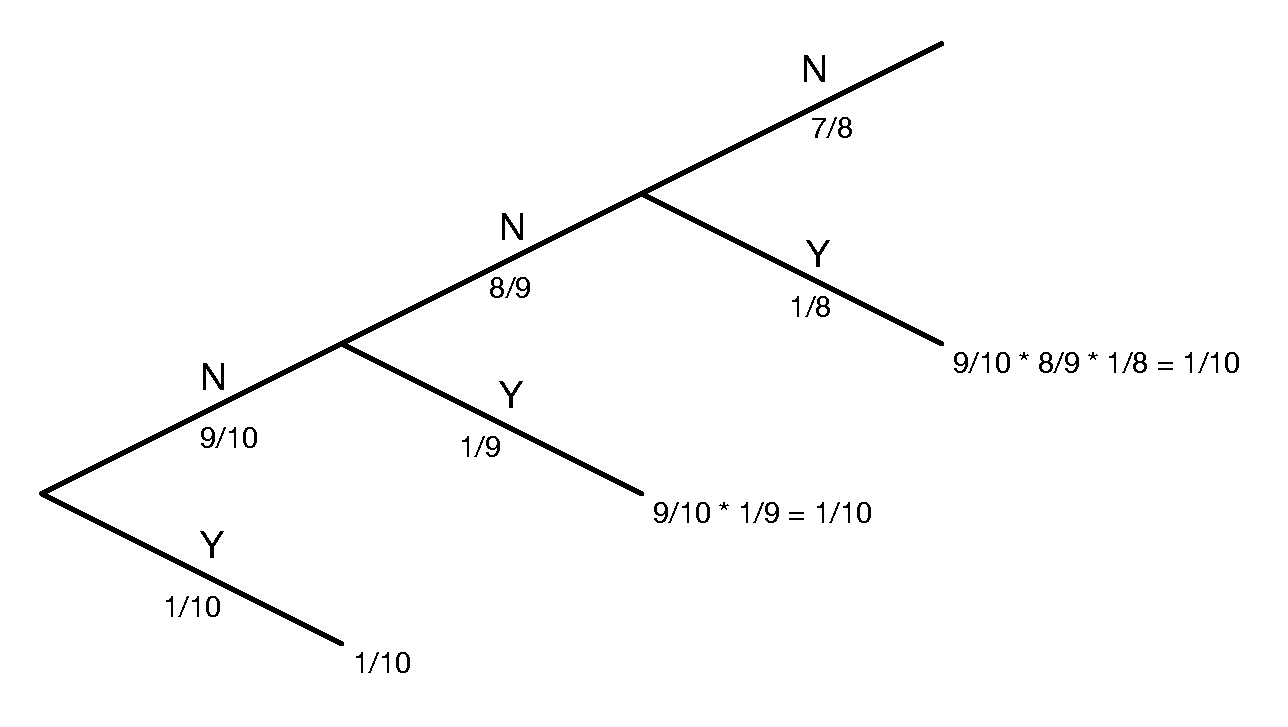
\includegraphics[width=10cm]{passwordtree}
\end{figure}
For the probability of getting it right on the first three tries, add up the branches that end in $Y$ to get
\[
\frac{1}{10} + \frac{1}{10} + \frac{1}{10} = \frac{3}{10} 
\]
Alternately, we can think of it this way. Indicating the results again by Y and N:
\begin{align*}
\P(\text{right in first three guesses}) = \P(Y) + \P(NY) + \P(NNY) \\
&= \frac{1}{10} + \frac{9}{10}\frac{1}{9} + \frac{9}{10}\frac{8}{9}\frac{1}{8}\\
&= \frac{3}{10}
\end{align*}
Note that the success probability \emph{increases} with each guess as you eliminate the unsuccessfull PINs from your list. If you were allowed 10 guesses, and the first 9 were incorrect, you would be \emph{guaranteed} to get it right on the last guess since you had narrowed the possibilities down to one by process of eliminiation. These are not Bernoulli trials, because the probability of success changes with each trial. Thus we cannot model this with a geometric distribution.

\item The eight Ivy-league schools (Brown, Columbia, Cornell, Dartmouth, Harvard, Penn, Princeton, and Yale) are having a badminton tournament. In the first round, the teams are paired off uniformly at random. How many possible outcomes are there for the first round? An ``outcome'' specifies both the team parings and the winners. Here is one such outcome:
\begin{figure}[H]
\centering
\fbox{\begin{minipage}{15em}
\begin{itemize}[noitemsep]
\item Brown beats Yale
\item Dartmouth beats Harvard
\item Princeton beats Penn
\item Columbia beats Cornell
\end{itemize}
\end{minipage}}
\end{figure}

I can think of at least two ways to do this, so I will show both of them.
\begin{enumerate}
\item This method uses multinomials. The first thing we will do is use the multinomial coefficient to divide the 8 teams in to four \emph{distinct} groups of 2. The number of ways to do this is
\[
\binom{8}{2\:2\:2\:2\:} = \frac{8!}{2!\:2!\:2!\:2!}
\]
We can think of this as dividing the teams into a first group, a second group, a third group, and a fourth group. In other words, when we use the multinomial, order matters! But we don't want order to matter, since all we care is who plays whom. To make order not matter, we divide by the number of ways of permuting the 4 groups, which is $4!$. So the number of pairings, where order does not matter, is:
\[
\dfrac{ \binom{8}{2\:2\:2\:2\:} } {4!} = \frac{8!}{4!\:2!\:2!\:2!\:2!}
\]
Now we need to account for the result of each match. For each match, there are two possible outcomes. Each of the possible pairings involves 4 matches. So for each pairing, there are $2 \cdot 2 \cdot 2 \cdot 2 = 2^4$ possible outcomes. Thus to get the total number of possible outcomes, we multiply the number of pairings by the number of outcomes per pairing to get:
\[
\frac{8!}{4!\:2!\:2!\:2!\:2!} 2^4 = \frac{8!}{4!}
\]

\item Another way to think of this is with permutations. For convenience, we will designate the teams by the letters A - H. Let's form strings from the 8 letters. There are $8!$ strings composed of the letters A - H since all letters are distinct and order matters. Let's look at one of them. Consider the string \texttt{ABCDEFGH} and write it with dividers as:
\[
\texttt{AB}|\texttt{CD}|\texttt{EF}|\texttt{GH}
\]
Let's call the things separated by dividers ``bins''. We will say that this denotes the outcome: A beats B, C beats D, E beats F, G beats H. But we can swap around the pairs, and get the same outcome. For example, the string
\[
\texttt{CD}|\texttt{AB}|\texttt{EF}|\texttt{GH}
\]
specifies the same outcome. How many different strings correspond to the same outcome? We can swap around the bins however we want without affecting the outcome. Since there are $4!$ ways to permute the 4 bins, we divide by $4!$ to get
\[
\frac{8!}{4!}
\]
total outcomes.

\end{enumerate}

\item You are the quality control manager for the Acme Widget Company. You have three factories which produce widgets. The table below gives the fraction of the total widget production allotted to each factory as well as the fraction of defective widgets produced by each factory.

\begin{figure}[H]
\centering
\begin{tabular}{lll}
\toprule
Factory & Fraction of total production & Fraction of defective widgets \\
\midrule
A & 0.20 & 0.020 \\
B & 0.30 & 0.010 \\
C & 0.50 & 0.005 \\
\bottomrule
\end{tabular}
\end{figure}
You test a randomly-selected widget and find that it is defective. What is the probability that it came from Factory A?\\

Let $A$, $B$, $C$ be the events that the widget came from those factories, and let $E$ be the event that the widget is defective. We are looking for $\P(A|E)$ Then by Bayes' theorem and the law of total probability:
\begin{align*}
\P(A|E) &= \frac{ \P(E|A)\P(A) } { \P(E)} \\
&= \frac{ \P(E|A)\P(A) }{\P(E|A)\P(A) + \P(E|B)\P(B) + \P(E|C)\P(C) } \\
&= \frac{ 0.020 \cdot 0.20 }{ 0.020 \cdot 0.20 + 0.010 \cdot 0.30 + 0.005 \cdot 0.50 } \\
&= \frac{0.004}{0.0095} \approx 0.42
\end{align*}

\end{enumerate}
\end{document}

